%%
%% Prinzip von Cavalieri 2025_02_11 (phi@bms-w.ch)

\subsection{Das Prinzip von Cavalieri}\index{schiefe Körper}\index{Cavalieri}
Bonaventura Francesco Cavalieri (1598 – 1647)


\begin{tabular}{cp{115mm}}
  \raisebox{-32mm}{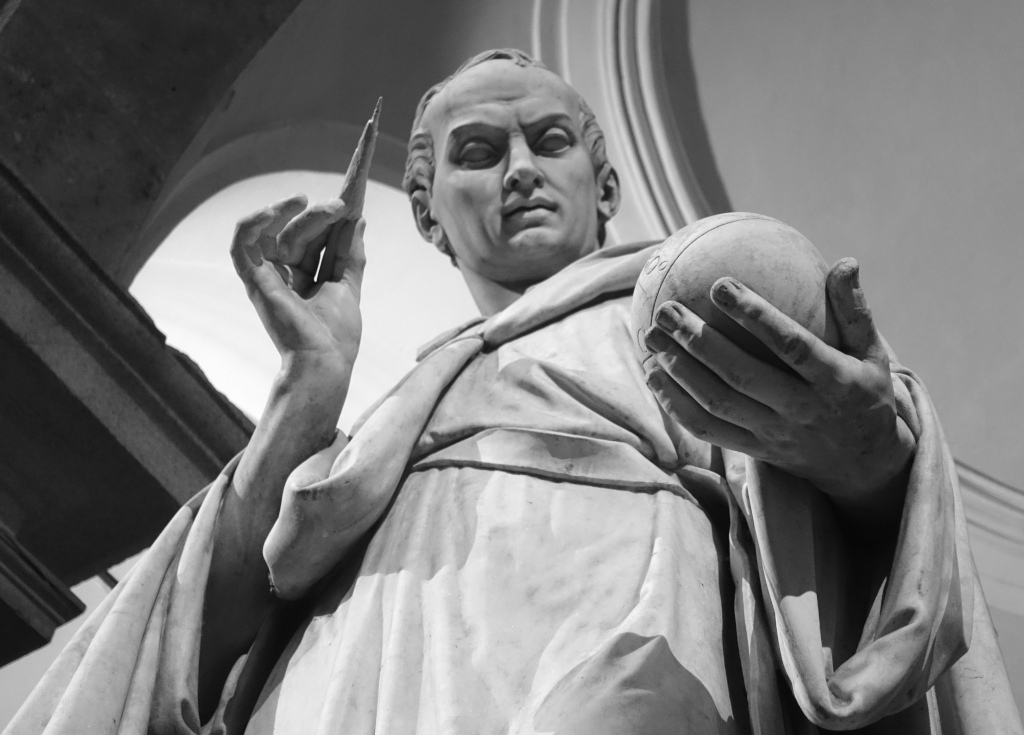
\includegraphics[width=50mm]{tals/stereo/img/cavalieri2.jpg}}\,\,
  &
  Das \textbf{Prinzip} sagt aus, dass zwei Körper das
selbe Volumen haben, genau dann, wenn sie in \textbf{jeder} horizontalen
Schnittebene die selbe Fläche aufweisen.

\\
\end{tabular}

{\footnotesize {Foto (Feb. 2025): Statue von Buonaventura
      Cavalieri, Milano, Brera-Museum}}



\TRAINER{Vorzeigen: Dies kann gut mit einem Stapel Jasskarten veranschaulicht
  werden, der in verschiedene Lagen geschert und «rotiert» wird.}

\vspace{4mm}

Das Prinzip an drei Körpern veranschaulicht:

\bbwCenterGraphic{178mm}{tals/stereo/img/Cavalieri.png}
Bildquelle: \texttt{www.slideshaer.net} (Mai 2021)
\vspace{9mm}

\begin{gesetz}{schiefe Körper}{}
  Schiefe Körper haben das selbe Volumen, wie der entsprechende gerade Körper, dabei wird die Höhe $h$ auch hier als Abstand zwischen Grund- und Deckflächenebene verwendet.

  $$ V = \frac13 \cdot{} \left(G + \sqrt{GD} + D \right) \cdot{} h $$
\end{gesetz}

\newpage
